\documentclass[11pt,letterpaper]{article}
\usepackage[lmargin=1in,rmargin=1in,tmargin=1in,bmargin=1in]{geometry}
\usepackage{../style/homework}
\usepackage{../style/commands}
\setbool{quotetype}{true} % True: Side; False: Under
\setbool{hideans}{false} % Student: True; Instructor: False

% -------------------
% Content
% -------------------
\begin{document}

\homework{8: Due 10/25}{I'll never let go, Jack. I'll never let go.}{Rose DeWitt Bukater, Titanic \par (Shortly before letting go\dots)}

% Problem 1
\problem{10} Below are two charts giving information on survival/death for the April 15, 1912 sinking of the Titanic. 
        \begin{table}[h]
        \centering
        \scalebox{0.93}{%
        \begin{tabular}{|c|c|c|c|c||c|} \hline
         & Men & Women & Boys & Girls & Total \\ \hline 
         Survived & 338 & 316 & 29 & 27 & 710 \\ \hline
         Died & 1352 & 109 & 35 & 18 & 1514 \\ \hline \hline
         Total & 1690 & 425 & 64 & 45 & 2224 \\ \hline
        \end{tabular}} \hfill \scalebox{0.93}{\begin{tabular}{|c||c|c||c|} \hline
        & Survived & Died & Total \\ \hline \hline
        First Class Men & 57 & 118 & 175 \\ \hline
        First Class Women & 140 & 4 & 144 \\ \hline
        First Class Children & 5 & 1 & 6 \\ \hline
        Second Class Men & 14 & 154 & 168 \\ \hline
        Second Class Women & 80 & 13 & 93 \\ \hline
        Second Class Children & 24 & 0 & 24 \\ \hline
        Third Class Men & 75 & 387 & 462 \\ \hline
        Third Class Women & 76 & 89 & 165 \\ \hline
        Third Class Children & 27 & 52 & 79 \\ \hline
        Crew (Men) & 192 & 693 & 885 \\ \hline
        Crew (Women) & 20 & 3 & 23 \\ \hline \hline
        Total & 710 & 1514 & 2224 \\ \hline
        \end{tabular}}
        \end{table}

\begin{enumerate}[(a)]
\item Find the probability that a randomly selected person died. 
\item Find the probability that a randomly selected person was a woman that died. 
\item Find the probability that a person that died was in first class. 
\item Find the probability that a person died or was in first class.
\item Find the probability that a person was a crew member. 
\end{enumerate} \pspace

\sol 
\begin{enumerate}[(a)]
\item 
	\[
	P(\text{died})= \dfrac{1514}{2224} \approx 0.680755
	\]

\item 
	\[
	P(\text{woman and died})= \dfrac{109}{2224} \approx 0.0490108
	\]

\item 
	\[
	P(\text{first class} \;|\; \text{died})= \dfrac{118 + 4 + 1}{1514}= \dfrac{123}{1514} \approx 0.0812417
	\]

\item 
	\[
	P(\text{died or first class})= \dfrac{(1514 + 175 + 144 + 6) - (118 + 4 + 1)}{2224}= \dfrac{1839 - 123}{2224}= \dfrac{1716}{2224} \approx 0.771583
	\]

\item 
	\[
	P(\text{crew})= \dfrac{885 + 23}{2224}= \dfrac{908}{2224} \approx 0.408273
	\]
\end{enumerate}


\newpage



% Problem 2
\problem{10} Some construction companies work exclusively with large businesses constructing office spaces, warehouses, etc. Others work in residential construction, and some work in both. Suppose that 47\% of construction companies work in business construction, 35\% of companies work in residential construction, and 12\% work in either area. 
        \begin{enumerate}[(a)]
        \item Find the percentage of companies that work in business or residential construction.
        \item Find the percentage of companies that work in neither business nor residential construction.
        \item Find the percentage of companies that work exclusively in business construction.
        \item Find the percentage of companies that work in residential construction that also do business construction.
        \item Find the percentage of companies that work exclusively in business or residential construction. 
        \end{enumerate} \pspace

\sol 
\begin{enumerate}[(a)]
\item 
	\[
	P(\text{business or residential})= 35\% + 12\% + 23\%= 70\%
	\]

\item 
	\[
	P(\text{neither business nor residential})= 30\%
	\]
 
\item 
	\[
	P(\text{only business})= 35\%
	\]
  
\item 
	\[
	P(\text{business} \;|\; \text{residential})= \dfrac{12\%}{12\% + 23\%}= \dfrac{12\%}{35\%} \approx 0.342857= 34.3\%
	\]
  
\item 
	\[
	P(\text{only business or only residential})= 35\% + 23\%= 58\%
	\] 
\end{enumerate} \vfill

	\[
	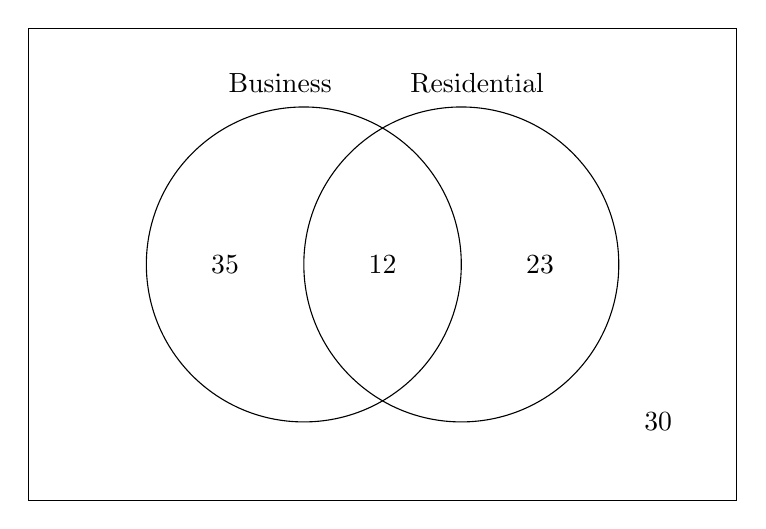
\begin{tikzpicture}
	\draw (0,0) rectangle (9,6);
	\draw (3.5,3) circle (2);
	\draw (5.5,3) circle (2);
	
	\node at (3.2,5.3) {Business};
	\node at (5.7,5.3) {Residential}; 
	
	\node at (2.5,3) {35};
	\node at (4.5,3) {12};
	\node at (6.5,3) {23};
	\node at (8,1) {30};
	\end{tikzpicture}
	\]



\newpage



% Problem 3
\problem{10} Suppose a disease only occurs in approximately 2\% of the population. A test is developed that detects this disease in those that have it 97\% of the time, and only incorrectly identifies those that do not have the disease as having it 4\% of the time. 
	\begin{enumerate}[(a)]
	\item Find the probability that a person tests positive for the disease. 
	\item Assuming independence, what is the probability that you test positive twice if you do not have the disease?
	\item Find the probability that a person has the disease or tests positive. 
	\item Find the probability that a person that tests positive for the disease actually has the disease. 
	\item Does your response in (d) contradict the fact that the test is `97\% accurate'? Explain. 
	\end{enumerate} \pspace

\sol 
\begin{enumerate}[(a)]
\item 
	\[
	P(\text{+})= 0.0194 + 0.0392= 0.0586
	\]

\item 
	\[
	P(\text{+ twice} \;|\; \text{Not})= P(\text{+} \;|\; \text{Not}) \cdot P(\text{+} \;|\; \text{Not})= \dfrac{0.0392}{0.98} \cdot \dfrac{0.0392}{0.98}= 0.0016
	\]

\item 
	\[
	P(\text{has or +})= 0.0194 + 0.0006 + 0.0392= 0.0592
	\]

\item 
	\[
	P(\text{has} \;|\; \text{+})= \dfrac{0.0194}{0.0194 + 0.03292}= \dfrac{0.0194}{0.0586}= 0.3311
	\]

\item No. We know that the test correctly identifies those with the disease as having the disease 97\% of the time. In that sense, the test is 97\% accurate. Similarly, it correctly identifies a person without the disease as not having it 96\% of the time. However accurate the test is, because the disease is `rare', if a positive test occurs it is more likely that it is one of these `rare' errors rather than actually being an indication of the disease. The test is `97\% accurate' as advertised. It is simply that a positive test result is more likely indicative of a `rare' error than a `rare' disease. 
\end{enumerate} \vfill

		\[
		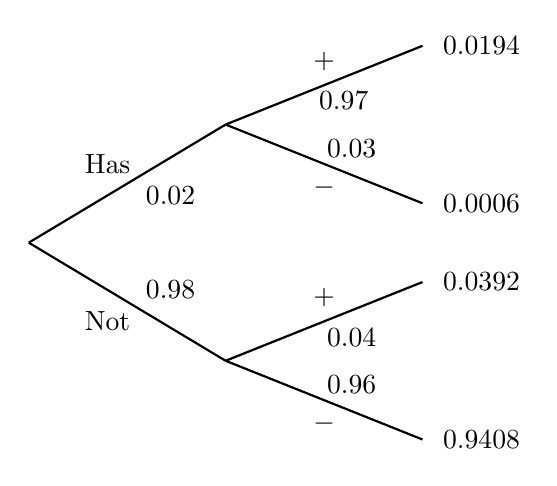
\begin{tikzpicture}[scale= 1.0]
		\def\FirstUpLabel{Has}
		\def\FirstDownLabel{Not}
		\def\SecondUpLabel{$+$}
		\def\SecondDownLabel{$-$}
		\def\Up{$0.02$}
		\def\Down{$0.98$}
		\def\UpUp{$0.97$}
		\def\UpDown{$0.03$}
		\def\DownUp{$0.04$}
		\def\DownDown{$0.96$}
		\def\first{$0.0194$}
		\def\second{$0.0006$}
		\def\third{$0.0392$}
		\def\fourth{$0.9408$}
		
		\node at (1,1) {\FirstUpLabel};	
		\node at (1,-1) {\FirstDownLabel};	
		\node at (1.8,0.6) {\Up};
		\node at (1.8,-0.6) {\Down};
		\draw[thick] (0,0) -- (2.5,1.5);
		\draw[thick] (0,0) -- (2.5,-1.5);
		
		\node at (3.75,2.3) {\SecondUpLabel};
		\node at (3.75,0.7) {\SecondDownLabel};
		\node at (4,1.8) {\UpUp};
		\node at (4.1,1.2) {\UpDown};
		\node at (5.75,2.5) {\first};
		\node at (5.75,0.5) {\second};
		\draw[thick] (2.5,1.5) -- (5,2.5);
		\draw[thick] (2.5,1.5) -- (5,0.5);

		\node at (3.75,-0.7) {\SecondUpLabel};
		\node at (3.75,-2.3) {\SecondDownLabel};
		\node at (4.1,-1.2) {\DownUp};
		\node at (4.1,-1.8) {\DownDown};
		\node at (5.75,-0.5) {\third};	
		\node at (5.75,-2.5) {\fourth};	
		\draw[thick] (2.5,-1.5) -- (5,-0.5);
		\draw[thick] (2.5,-1.5) -- (5,-2.5);
		\end{tikzpicture}
		\]


\end{document}